% =====================================================================
%  2026-05-18 — 設計第一版 PCB:PD_detector_pro (flico shield v1)
% =====================================================================

\subsection*{今日目標}

\begin{itemize}[leftmargin=2em,itemsep=0pt]
  \item 把 5/12 麵包板上的「BPW34 \(+\) MCP6002 TIA \(+\) 74HC4051 mux \(+\) Pico \(+\) OLED」
        這條訊號鏈轉成 PCB——但是\textbf{先做 first-version,不是要直接投產}。
  \item 借這版 PCB 把 \textbf{KiCad/SKiDL 設計流程}走一遍:選 0805 SMD 規格、
        綁 LCSC 編號、SKiDL 跑出 netlist、KiCad 匯入 + 用 Python (\texttt{pcbnew})
        程式化擺件、輸出 Gerber/BOM/CPL。整套流程下次設計第二版時可以直接重用。
  \item 順便對\textbf{元件規格做一次升級盤點}:從麵包板的 hobby-grade
        (MCP6002, 74HC4051, Pico ADC) 升到精密量測等級
        (OPA328, TMUX1208, 外接 ADS8326 16-bit SAR),
        確認規格升上去後 PCB 該長什麼樣。
\end{itemize}

\subsection*{為什麼是 \texttt{first-version} 不是 \texttt{v1.0}}

幾個還沒收斂的關鍵問題,故意留給之後的版本解:

\begin{itemize}[leftmargin=2em,itemsep=0pt]
  \item \textbf{感測器選型}:雖然麵包板是用 BPW34(便宜、好買),但 0518 討論時意識到
        \textbf{SFH 2440}(更接近人眼響應、低反向暗電流)更適合做螢幕閃爍量測。
        但 SFH 2440 是 \emph{top-looker} SMD 封裝,感光面垂直 PCB 出來,
        跟「裝在耳機盒底部、光從底面進」的機構配置直接衝突 —— 要嘛走 90 度導光柱
        (3D 印透明 PETG/壓克力),要嘛改型號。今天的版本先沿用 BPW34
        把佈線跑通,選型留到 v2 收尾。
  \item \textbf{外殼方向}:「耳機盒」造型(USB-C 朝上、感光口朝下、Pico 與 PCB 平行疊)
        的機構決策今天才定下來,3D 列印外殼還在 Fusion 360 裡半成品。
  \item \textbf{ADC 軟體鏈}:把採樣率拉到 \(\SI{32}{\kilo\hertz}\) 要靠 Pico 端
        SPI \(+\) hardware timer \(+\) USB binary stream,這條鏈得用 C++ Pico SDK
        重寫(5/12 已決定),但今天 host 端的 PyQtGraph dashboard 也還沒寫。
  \item \textbf{電池供電}:原本想做 LiPo 內建,但 OPA328 \(+\) TMUX1208 \(+\) ADS8326
        全要 \(\SI{3.3}{\volt}\) 純淨類比電源,USB 雜訊問題用 ferrite bead \(+\) LP5907 LDO
        解。電池路徑加上 MCP73831 充電 IC \(+\) SS14 蕭特基 OR-ing,目前已畫入 schematic
        但實體尚未在麵包板驗證,可能 v2 就把整段砍掉、改純 USB 供電。
\end{itemize}

所以這版定位是\textbf{流程驗證 + 規格盤點}:讓 SKiDL/pcbnew 工具鏈跑通,
把元件升級的影響真實畫到佈線上看,但不送 JLCPCB 投產。\textbf{歸檔在
\texttt{hardware/first-version/}。}

\subsection*{規格升級盤點}

對照麵包板原型(5/12 定稿)→ 這版 PCB:

\begin{table}[H]
  \centering
  \caption{flico 從麵包板原型升級到 first-version PCB 的元件規格盤點。}
  \label{tab:0518-spec}
  \small
  \begin{tabular}{lll}
    \toprule
    位置 & 麵包板版本 & first-version PCB 版本 \\
    \midrule
    Op-amp     & MCP6002 (DIP-8, 100\,pA $I_B$)
               & \textbf{OPA328} (SOT-23-5, 0.2\,pA $I_B$, RRIO, 3.3\,V) \\
    類比 mux   & 74HC4051 (8-ch, $R_\text{on}$\,$\approx$\,100\,\(\Omega\), \(I_\text{leak}\) ns\,nA)
               & \textbf{TMUX1208} (8-ch, $R_\text{on}$\,$\approx$\,5\,\(\Omega\), \(I_\text{leak}\) ns\,10\,pA) \\
    回授網路   & 4 檔 (1\,k / 10\,k / 100\,k / 1\,M)
               & \textbf{8 檔對數} (1\,k, 3.3\,k, 10\,k, 33\,k, 100\,k, 330\,k, 1\,M, 10\,M\(\Omega\)) \\
    回授補償 $C_f$ & 雜湊配對(1\,n / 330\,p / 33\,p / 1\,p)
               & 全部按 \(f_c=\SI{16}{\kilo\hertz}\) 重算:10\,n / 3.3\,n / 1\,n / 330\,p / 100\,p / 33\,p / 10\,p / 1\,p \\
    ADC        & Pico 內建 (12-bit, ENOB $\approx$ 9, 跟著數位雜訊)
               & \textbf{ADS8326} (外接 SPI, 16-bit SAR, 250\,kSps) \\
    電源       & Pico 3V3 直接餵類比
               & VBUS \(\to\) ferrite bead \(\to\) \textbf{LP5907} LDO \(\to\) +3V3\_A (類比專屬軌) \\
    接地       & 單一 GND
               & \textbf{Star grounding}:GND \(+\) GNDA 分離,LDO 旁邊 0\,\(\Omega\) 拼回 \\
    電池       & 不接(5/11 LiPo 還沒上)
               & MCP73831 充電 + SS14 OR-ing(畫進去但 v2 可能砍) \\
    顯示       & SSD1306 0.91" OLED via I\textsuperscript{2}C
               & 同上(複用 5/11 寫好的 \texttt{ssd1306.py}) \\
    \bottomrule
  \end{tabular}
\end{table}

關鍵理由:

\begin{itemize}[leftmargin=2em,itemsep=0pt]
  \item \textbf{OPA328 取代 MCP6002}:在 10\,M\(\Omega\) 高增益下,
        100\,pA 偏置電流會在輸出端疊出 \(\SI{1}{\milli\volt}\) 偏置 + 漂移;
        0.2\,pA 直接降 500 倍,基本上是測量極限的天花板。
  \item \textbf{TMUX1208 取代 74HC4051}:
        \(R_\text{on}\) 從 100\,\(\Omega\) 降到 5\,\(\Omega\),在 1\,k\(\Omega\) 檔位的增益誤差
        從 10\% 降到 0.5\%;漏電流降 100 倍,10\,M\(\Omega\) 檔位的偏置誤差從
        \(\sim 10\,\mathrm{mV}\) 降到不到 \(\SI{1}{\micro\volt}\)。
  \item \textbf{8 檔對數 \(R_f\)}:1\(\to\) 10 跳階(4 檔)會在中間出現
        「上一檔太弱、下一檔已飽和」的死區;改 \(1 \to 3.3 \to 10\) (E12 序列、8 檔)
        可以無縫覆蓋 \(10^7\) dynamic range,自動換檔的 hysteresis 變得更平順。
  \item \textbf{每檔 \(C_f\) 按 \(f_c = \SI{16}{\kilo\hertz}\) 收歛}:
        \(C_f = 1 / (2\pi f_c R_f)\)、目標 Nyquist 截止跟採樣率對齊。
        從原本「能塞什麼塞什麼」改成正規 anti-alias filter,所有檔位的頻寬都對齊在
        \(\sim \SI{16}{\kilo\hertz}\),量測一致性提升。
  \item \textbf{外接 ADS8326 取代內建 ADC}:RP2040 內建 ADC 的 INL/DNL 鋸齒誤差
        已知會把 ENOB 拉到 \(\sim 9\) bit,加上跟 Pico 數位電路共電的雜訊,
        12-bit 名義上的精度根本拿不到;外接 16-bit SAR 直接給乾淨的 65,536 階。
  \item \textbf{LP5907 LDO + ferrite bead + 星型接地}:
        Pico 的 3V3 是 buck 出來的、有 \(\sim \mathrm{kHz}\) ripple;
        要做精密類比就得有一條獨立的、跟數位地解耦的 +3V3\_A。
\end{itemize}

\subsection*{設計流程:SKiDL \(\to\) Netlist \(\to\) KiCad \(\to\) Python \texttt{pcbnew} 自動擺件}

KiCad 8/10 的原生流程是 GUI:在 Schematic Editor 拉線、annotate、選 footprint、
按 F8 (\emph{Update PCB from Schematic})、在 PCB Editor 手動擺件。今天決定走 \textbf{程式化}
路線,理由是:這版會反覆改規格,GUI 重畫很煩、版本控制(看 diff)也痛苦。

\begin{itemize}[leftmargin=2em,itemsep=0pt]
  \item \textbf{Schematic}:用 \textbf{SKiDL}(Python DSL for schematics)寫\\
        \texttt{hardware/first-version/gen\_schematic.py}。元件用 \texttt{Part("Device", "R", ...)}
        宣告,連線用 Python \texttt{Net} 物件 \texttt{+=}。
        產出 \texttt{pd\_detector.net}(KiCad netlist 格式)。
  \item \textbf{Footprints 綁 LCSC}:SKiDL 元件加自定義欄位
        \texttt{LCSC=Cxxxxx} 直接寫進 BOM(56k 0805 \(\to\) C17414、
        SS14 \(\to\) C8601、MCP73831 \(\to\) C116490 …… ),
        JLCPCB 下單時不會問「這是哪一顆」。
  \item \textbf{Import 到 KiCad}:在 PCB Editor → \emph{File} → \emph{Import} → \emph{Netlist},
        指 \texttt{pd\_detector.net}。所有元件 footprint 一次跑到畫布,
        ratsnest(白色飛線)就是設計連線的全部 ground truth。
  \item \textbf{擺件靠 \texttt{pcbnew} Python API}:寫
        \texttt{hardware/first-version/apply\_layout.py},
        用座標把元件 一顆顆 \(\texttt{SetPosition(VECTOR2I\_MM(x, y))}\),
        透過 KiCad 內建的 Python 直譯器執行
        (路徑:\texttt{/Applications/KiCad/KiCad.app/Contents/Frameworks/Python.framework/.../python3})。
        改一個座標 \(\to\) 跑一次腳本 \(\to\) KiCad GUI \emph{Reload from Disk} \(\to\) 看結果,
        比拖 GUI 快 5\(\times\) 以上,而且版本控制看得到 diff。
  \item \textbf{rendering 出圖}:寫 \texttt{reset\_routing.py} 把線清乾淨重畫;
        SVG/PNG 渲染存在 \texttt{layout\_renders/} 給日記引用(圖~\ref{fig:0518-top-tia}~\ref{fig:0518-top}~\ref{fig:0518-island})。
\end{itemize}

\subsection*{關鍵架構決策:flipped analog island}

排到一半 Claude Code 跑出個 plan,把 D1(BPW34/SFH 2440)搬到 PCB 最下緣(\(Y=48.5\) mm,
靠近耳機盒底部光口),但把 TIA 那一塊(U2 OPA328、U3 TMUX1208、八檔 \(R_f / C_f\))留在板子中間(\(Y \approx 19.5\) mm)。我覆盤了一下,這個排法\textbf{表面合理但物理上致命}:

\begin{itemize}[leftmargin=2em,itemsep=0pt]
  \item \texttt{TIA\_SUM} net(光二極體陰極 \(\to\) op-amp \(V^-\))會橫跨 PCB 接近 30 mm。
  \item 在 \(R_f = 10\,\mathrm{M}\Omega\) 的高增益下,這 30 mm 銅箔就是一根超級天線,
        \(\SI{60}{\hertz}\) 市電雜訊會被吸進去放大七位數倍。
  \item Trace 自帶 \(\sim 0.5\,\mathrm{pF/cm}\) 寄生電容 \(\Rightarrow\) 30 mm \(\approx\) 1.5 pF \(\Rightarrow\)
        \(R_f = 10\,\mathrm{M}\Omega\) 那檔頻寬從 \(\SI{32}{\kilo\hertz}\) 掉到 \(\SI{25}{\kilo\hertz}\),
        甚至誘發 op-amp 震盪(因為 \(C_\text{in} + C_\text{parasitic}\) 超過相位 margin)。
\end{itemize}

對策:整塊\textbf{類比 island 一起翻到板底},D1 跟 TIA 貼緊放(\(Y = 35 \sim 48\) mm),
數位 ADC + decoupling 移到上半板(\(Y = 5 \sim 30\) mm)。\texttt{TIA\_SUM} 走線
壓到 \(\sim 3\) mm。代價是 SPI 那邊 trace 變長,但 SPI 是數位邏輯訊號、
雜訊容忍度高得多,完全可以接受。

\begin{figure}[H]
  \centering
  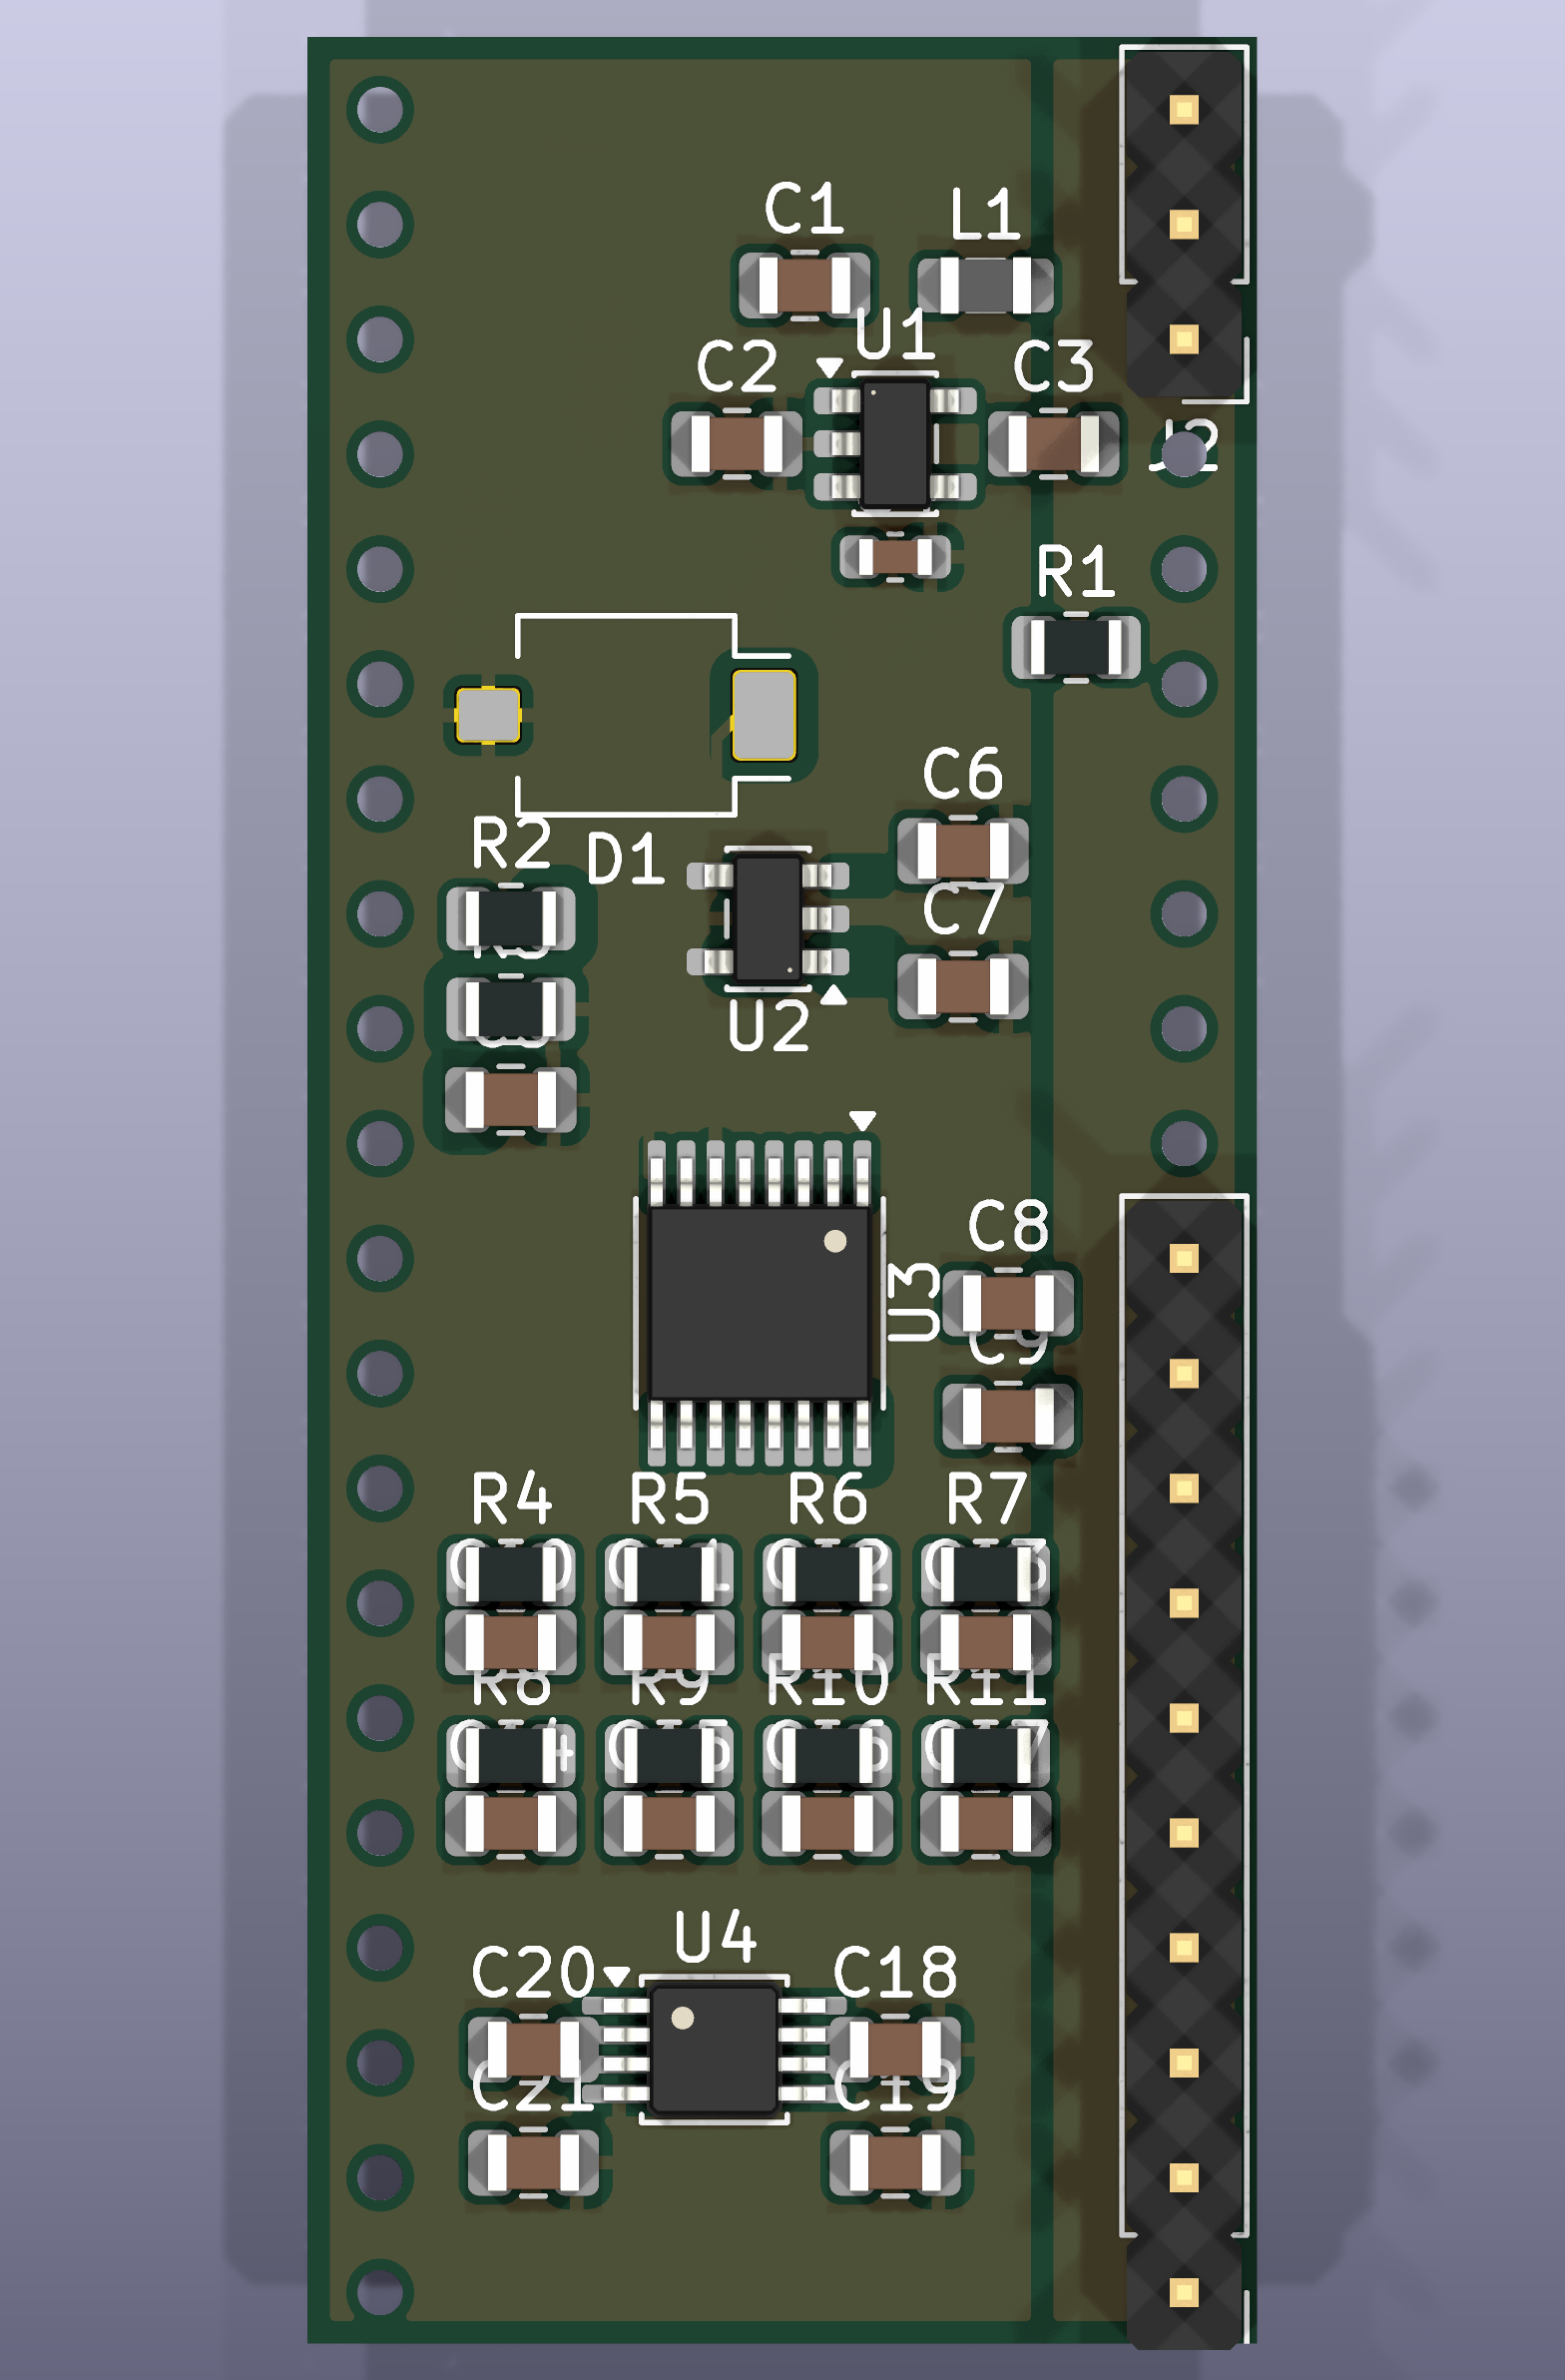
\includegraphics[width=0.7\linewidth]{2026-05-18/top_tia_sum.png}
  \caption{TIA 區塊放大渲染(top.svg 局部):op-amp(U2)、TMUX1208(U3)、
           八檔 \(R_f / C_f\) 全部緊靠 D1,\texttt{TIA\_SUM} 走線壓到 \(< 5\) mm。
           feedback 電容 \(C_f\) 跟 \(R_f\) 同點接,
           anti-alias filter 形成一致的 \(\sim \SI{16}{\kilo\hertz}\) 截止。}
  \label{fig:0518-top-tia}
\end{figure}

\begin{figure}[H]
  \centering
  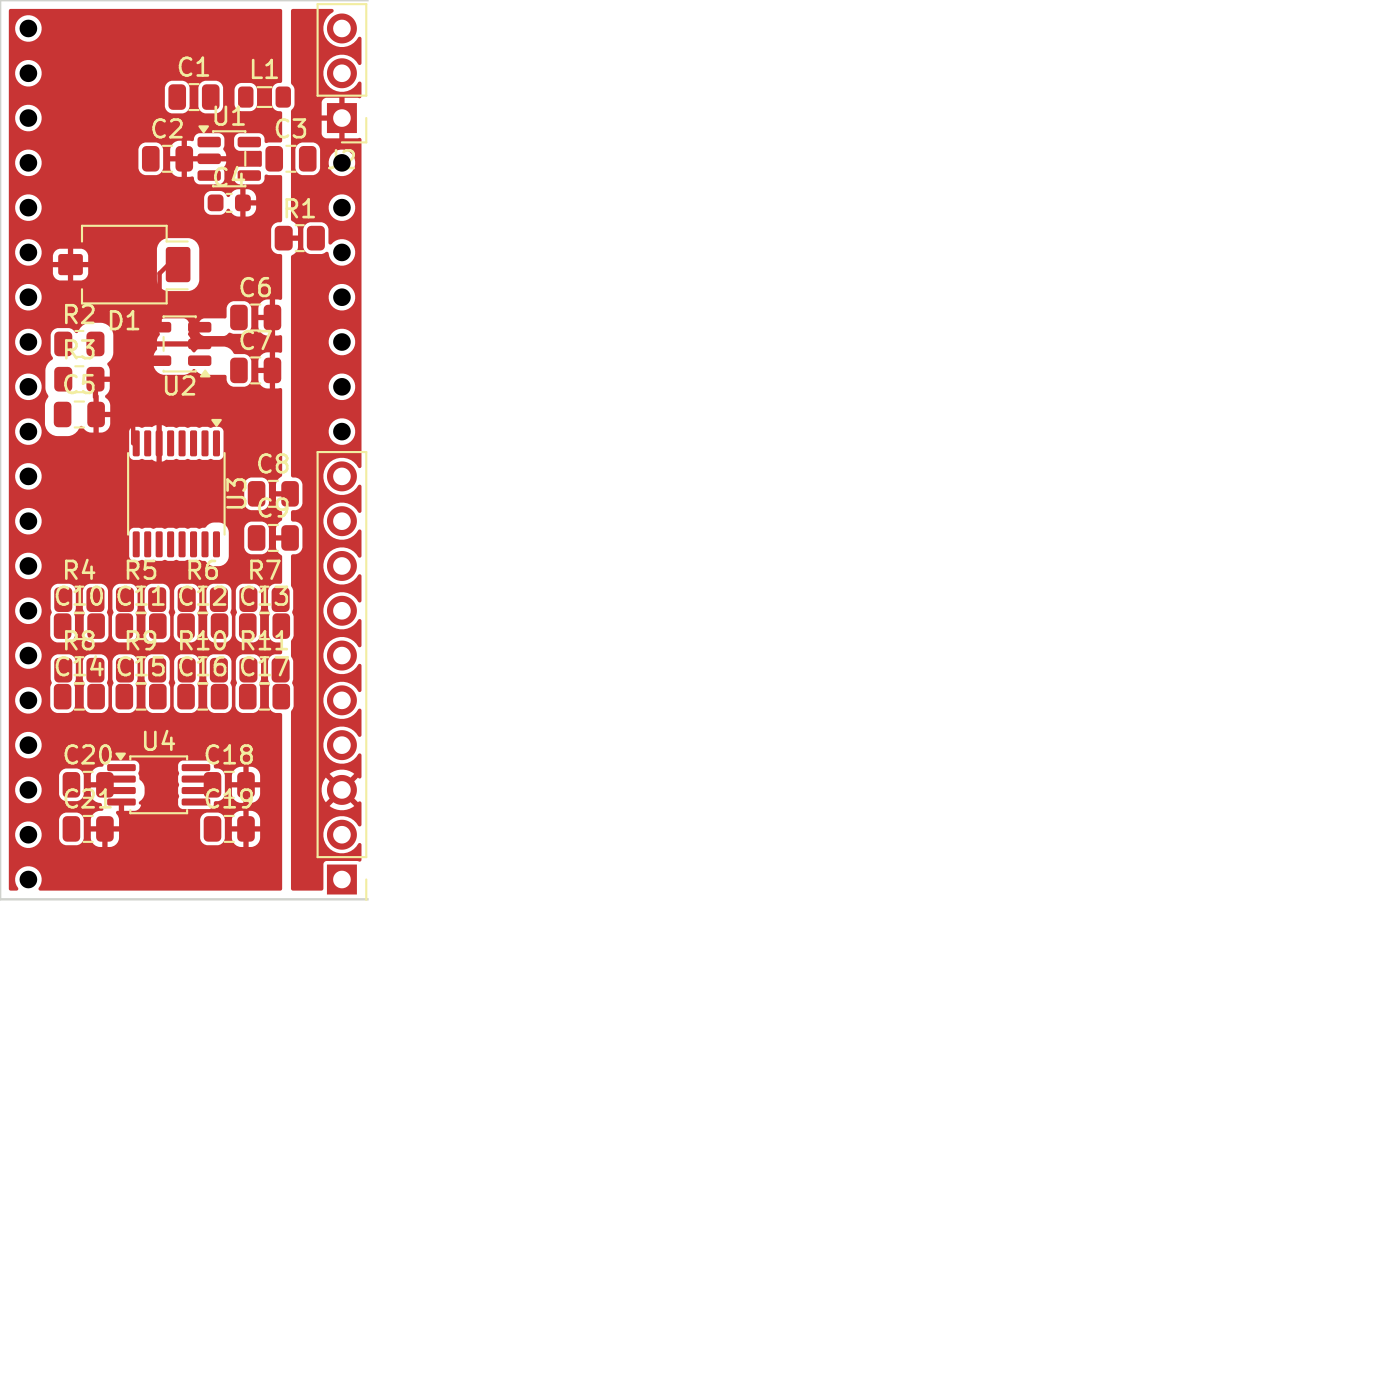
\includegraphics[width=0.85\linewidth]{2026-05-18/top.svg.png}
  \caption{flipped island 架構全板正面渲染。下半:類比安靜區(BPW34 D1
           + OPA328 TIA + TMUX1208 mux + 八檔 \(R_f / C_f\) + V\_REF 偏壓分壓)。
           上半:數位區(LP5907 LDO + ADS8326 SPI ADC + Pico header + MCP73831 充電)。
           中段 0\,\(\Omega\) 拼接點 = star ground,GND 跟 GNDA 在這唯一相連。}
  \label{fig:0518-top}
\end{figure}

\begin{figure}[H]
  \centering
  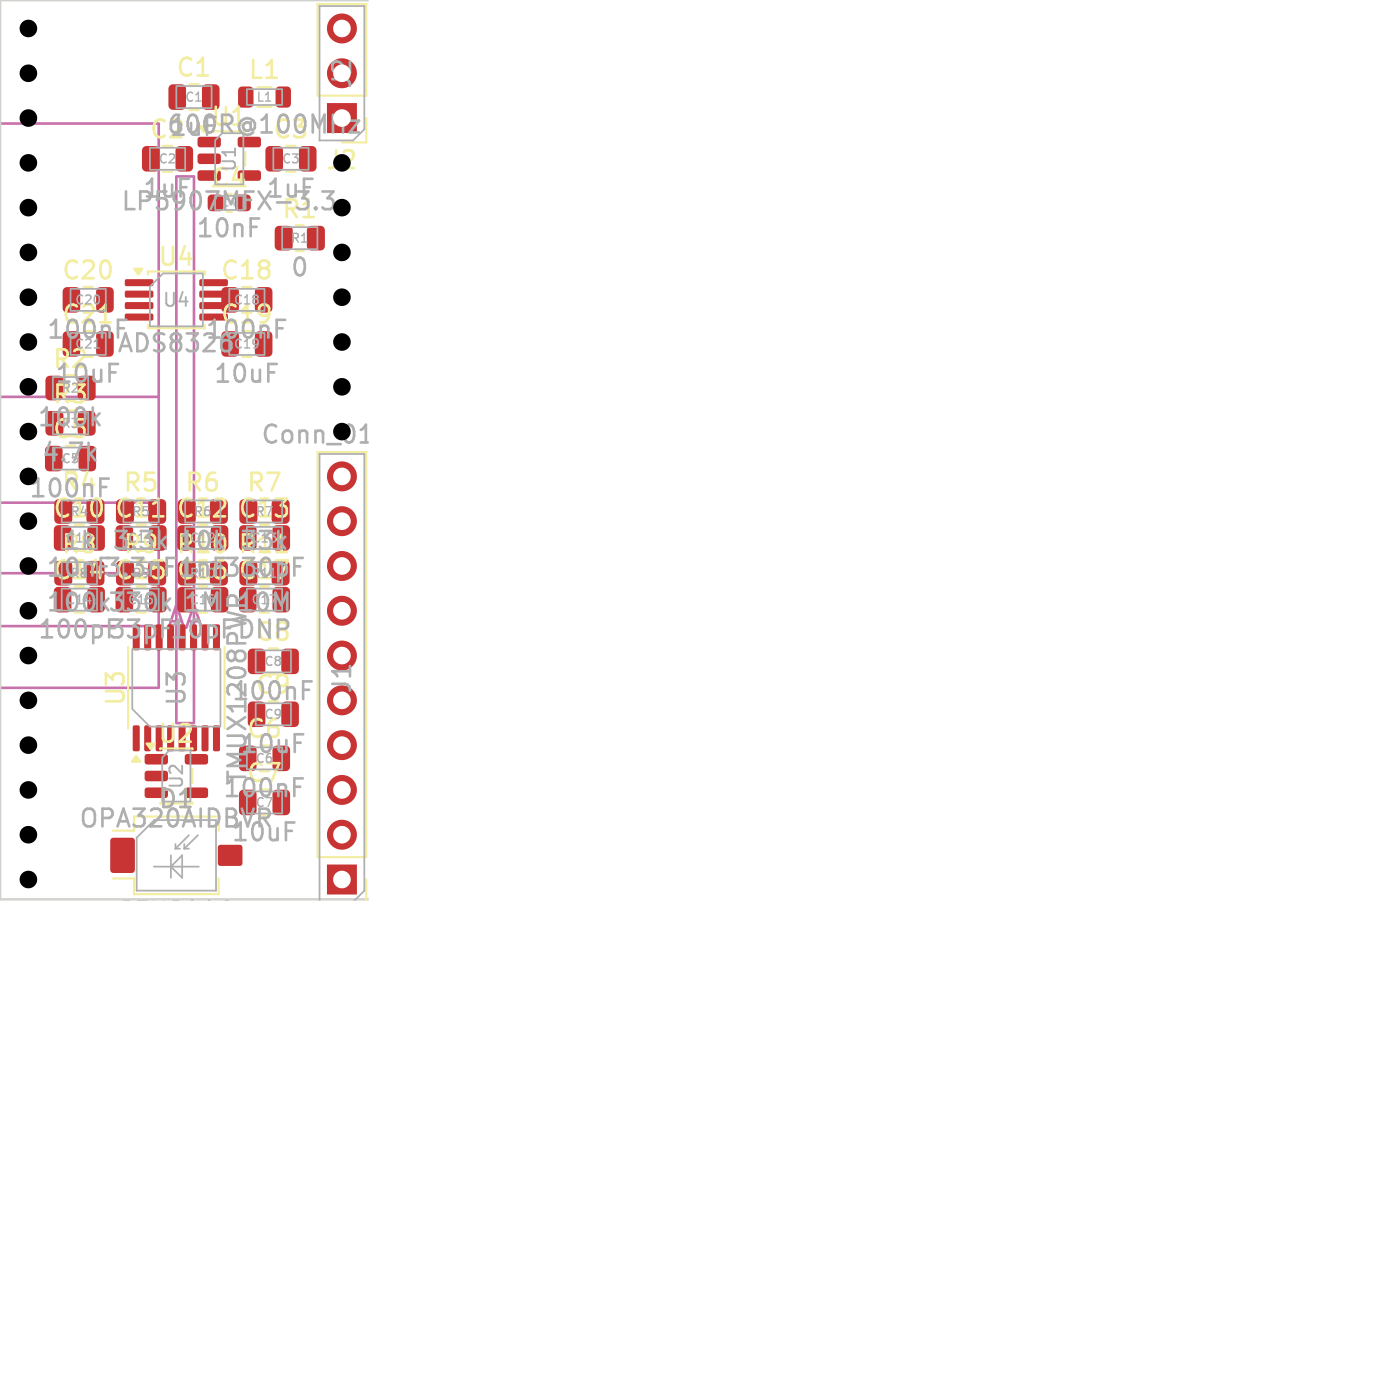
\includegraphics[width=0.7\linewidth]{2026-05-18/flipped_island.svg.png}
  \caption{flipped island 配置示意:把 D1(光感)從上方搬到下方,
           整塊 TIA 跟著翻轉,讓 \texttt{TIA\_SUM} 走線縮到最短。
           原本「ADC 在下、TIA 在上」是配合 USB-C/Pico 走線方便,
           但物理上犧牲了類比 SNR。}
  \label{fig:0518-island}
\end{figure}

\subsection*{順手解掉的細節}

過程中還塞了好幾個 0518 跟 Gemini/Claude 來回討論時學到的東西:

\begin{itemize}[leftmargin=2em,itemsep=0pt]
  \item \textbf{C0G/NP0 陶瓷材質}:八檔 \(C_f\) 都要 C0G/NP0,
        \textbf{不能用 X7R/Y5V} —— 後者有壓電效應,外殼震動會在 10\,M\(\Omega\)
        高增益下被放大成雜訊。
  \item \textbf{Mux common 接 \(V^-\) 不接 \(V_\text{out}\)}:把 TMUX1208 的 COM 接到
        op-amp 反相輸入(虛擬接地點)而非輸出端 —— 因為 mux 內部約 25 pF 寄生電容,
        如果掛在輸出端,會隨著 \(V_\text{out}\) 大幅充放電產生失真;掛在虛擬接地點電位幾乎不變,
        雜訊影響最小。
  \item \textbf{Power path}:USB \(\to\) D2 蕭特基 \(\to\) Pico VSYS;
        Battery \(\to\) D4 蕭特基 \(\to\) Pico VSYS;
        兩條 OR-ing。MCP73831 的 PROG 腳要 2\,k\(\Omega\) 到 GND 設充電電流 \(\sim 500\) mA。
        STAT 是 open-drain,LED 要接到 VBUS 上 \(\to\) 電阻 \(\to\) LED \(\to\) STAT,不能反過來。
  \item \textbf{ERC PWR\_FLAG}:KiCad ERC 會把
        \emph{Input Power pin not driven by any Output Power pins} 紅標出來。
        要在 VSYS 跟 GND/GNDA 各接一個 PWR\_FLAG,跟它說「這條線是真的有電的」。
  \item \textbf{打 via 規則}:\texttt{TIA\_SUM} 絕對不打 via(via 自帶 \(\sim 0.3\) pF 寄生 +
        阻抗不連續,10\,M\(\Omega\) 高增益下會放大);電源跟 GNDA 可以多打、
        孔徑也可以大(0.4 mm drill / 0.8 mm size)降低迴路阻抗。
\end{itemize}

\subsection*{產物 \(+\) 留檔}

當天的設計 commit 到 \texttt{hardware/first-version/}:

\begin{itemize}[leftmargin=2em,itemsep=0pt]
  \item \texttt{gen\_schematic.py}(\(\sim 300\) 行,SKiDL DSL) + \texttt{gen\_schematic\_sklib.py}
        (cache 的元件 symbol)
  \item \texttt{pd\_detector.net}(40 KB,KiCad netlist 格式 — schematic 的 ground truth)
  \item \texttt{PD\_detector\_pro.kicad\_pro / .kicad\_pcb / .kicad\_sch / .kicad\_prl}
        (PCB editor 專案;\texttt{.kicad\_sch} 是空 stub,因為 schematic 由 SKiDL 直接生 netlist,
        沒有 GUI schematic)
  \item \texttt{apply\_layout.py}(\(\sim 600\) 行,pcbnew API 程式化擺件) +
        \texttt{reset\_routing.py}(\(\sim 200\) 行,清線重畫)
  \item \texttt{gen\_schematic.erc / .log}(SKiDL 跑出來的 ERC 報告)
  \item \texttt{layout\_renders/}(top.svg / .png、flipped\_island.svg / .png、top\_tia\_sum.png)
\end{itemize}

\textbf{完整的 0518 Gemini 對話檔}留在
\texttt{report/research-log/gemini\_discuss\_history/0518.txt}(\(\sim 5000\) 行)——
從 0805 封裝選型、JLCPCB PCBA 流程、MCP73831 vs TP4056、LiPo 採購、I\textsuperscript{2}C OLED、
74HC4051 接線、SKiDL 跟 KiCad 整合、TMUX1208/OPA328/ADS8326 升級、抗混疊濾波公式、
flipped island 決策一路討論到 via 規則,完整重現整天設計思路。

\subsection*{今日心得}

\begin{itemize}[leftmargin=2em,itemsep=0pt]
  \item \textbf{先把流程跑通比先把規格定死重要}。元件選 OPA328 還是 OPA140、
        電池要不要進、SFH 2440 還是 BPW34,這些今天都沒最終定案 ——
        但 SKiDL \(+\) pcbnew Python API 這條\textbf{自動化設計流程}先跑通,
        下次改規格就只改幾行 Python,不用重新滑滑鼠拖 GUI。
  \item \textbf{flipped island 是今天最大的 architectural insight}。如果直覺照「Pico 朝上、
        D1 朝下」排,TIA 會掛在中間 \(\to\) \texttt{TIA\_SUM} 30 mm \(\to\) 板子當天線。
        類比設計的鐵律就是「敏感的東西盡量短盡量靠近」,要為了這個翻整塊 island 也得翻。
  \item \textbf{SKiDL 的最大好處不是寫起來快,是 review 起來快}。Schematic 變成 Python code,
        \texttt{git diff} 就能看見「上次到這次改了哪一條 net、加了哪顆元件」。
        對於 \textbf{Gemini/Claude 來回提案修改}的 workflow,文字 diff 不可或缺。
  \item \textbf{下一步}:
        \begin{enumerate}[leftmargin=2em,itemsep=0pt]
          \item \textbf{不打板。} 規格還沒收斂,直接送 JLCPCB 等於燒錢。
                把所有「待解」項目(感測器選型、SFH 2440 機構問題、電池要不要進、
                C++ ADC 鏈)各自獨立解掉,再做 v2。
          \item C++ firmware 主線(5/12 fork 出來那條)繼續推:
                ADC + PIO + DMA \(\to\) ring buffer,目標 \(\SI{32}{\kilo\hertz}\) jitter-free。
          \item Host 端 \texttt{host/} 寫 PyQtGraph 即時 dashboard,
                吃 USB binary stream + FFT + 自動跟著 Pico 的 GAP marker。
          \item 開始畫 3D 列印外殼(Fusion 360),確認 SFH 2440 光路要走導光柱
                還是側焊 — 機構決定回頭影響感測器選型。
        \end{enumerate}
\end{itemize}
